%# Στοιχεία αρχείου Pithanothtes-Table-Endexomena--------
\begin{longtable}{c>{\centering}m{2.5cm}>{\centering}m{5cm} c}
\hline \rule[-2ex]{0pt}{5.5ex} \textbf{Συμβολισμός} & \textbf{Ενδεχόμενο} & \textbf{Περιγραφή} & \textbf{Διάγραμμα} \\ 
\hhline{====} \rule[-2ex]{0pt}{8.5ex} $ x\in A $ & Ενδεχόμενο Α & Το ενδεχόμενο $ Α $ πραγματοποιείται. & \parbox[c]{22mm}{\mbox{}\\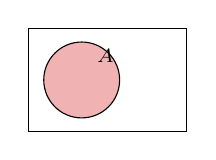
\begin{tikzpicture}[scale=.438]
\draw (-2,-2) rectangle (2.6,1);
\scope % A \cap B
\fill[red!80!black!30] (-.45,-.5) circle (1.1);
\draw[black] (-.45,-.5) circle (1.1);
\endscope
\tkzText(-1.6,-1.6){{\scriptsize $ \varOmega $}}
\tkzText(-.45,.1){{\scriptsize $ A $}}
\end{tikzpicture}} \\ 
\rule[-2ex]{0pt}{8.5ex} $ x\in A' $ & Συμπλήρωμα του $ A $ & Το ενδεχόμενο $ A $ \textbf{δεν} πραγματοποιείται. & \parbox[c]{22mm}{\mbox{}\\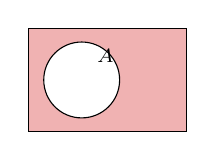
\begin{tikzpicture}[scale=.438]
\filldraw[fill=red!80!black!30] (-2,-2) rectangle (2.6,1);
\scope % A \cap B
\fill[white] (-.45,-.5) circle (1.1);
\draw[black] (-.45,-.5) circle (1.1);
\endscope
\tkzText(-1.6,-1.6){{\scriptsize $ \varOmega $}}
\tkzText(-.45,.1){{\scriptsize $ A $}}
\end{tikzpicture}} \\ 
\rule[-2ex]{0pt}{8.5ex} $ x\in A\cup B $ & Ένωση του $ A $ με το $ B $ & Πραγματοποιείται ένα \textbf{τουλάχιστον} από τα ενδεχόμενα $ A $ και $ B $. & \parbox[c]{22mm}{\mbox{}\\\begin{venndiagram2sets}[tikzoptions={scale=.4},shade=red!80!black!30,labelA={{\scriptsize $ A $}},labelB={{\scriptsize $ B $}},labelNotAB={{\scriptsize $ \varOmega $}}]
\fillA \fillB
\end{venndiagram2sets}} \\ 
\rule[-2ex]{0pt}{8.5ex} $ x\in A\cap B $ & Τομή του $ A $ με το $ B $ & Πραγματοποιούνται \textbf{συγχρόνως} τα ενδ. $ A $ και $ B $. & \parbox[c]{22mm}{\mbox{}\\\begin{venndiagram2sets}[tikzoptions={scale=.4},shade=red!80!black!30,labelA={{\scriptsize $ A $}},labelB={{\scriptsize $ B $}},labelNotAB={{\scriptsize $ \varOmega $}}]
\fillACapB
\end{venndiagram2sets}} \\ 
\rule[-2ex]{0pt}{8.5ex} $ x\in A-B $ & Διαφορά του $ B $ απ' το $ A $ & Πραγματοποιείται \textbf{μόνο} το ενδεχόμενο $ A $. & \parbox[c]{22mm}{\mbox{}\\\begin{venndiagram2sets}[tikzoptions={scale=.4},shade=red!80!black!30,labelA={{\scriptsize $ A $}},labelB={{\scriptsize $ B $}},labelNotAB={{\scriptsize $ \varOmega $}}]
\fillANotB
\end{venndiagram2sets}} \\ 
\rule[-2ex]{0pt}{8.5ex} $ x\in B-A $ & Διαφορά του $ A $ απ' το $ B $ & Πραγματοποιείται \textbf{μόνο} το ενδεχόμενο $ B $. & \parbox[c]{22mm}{\mbox{}\\\begin{venndiagram2sets}[tikzoptions={scale=.4},shade=red!80!black!30,labelA={{\scriptsize $ A $}},labelB={{\scriptsize $ B $}},labelNotAB={{\scriptsize $ \varOmega $}}]
\fillBNotA
\end{venndiagram2sets}} \\ 
\rule[-2ex]{0pt}{8.5ex} $ x\in\left(A-B\right)\cup\left(B-A\right) $ & Ένωση διαφορών & Πραγματοποιείται \textbf{μόνο} ένα από τα δύο σύνολα (ή μόνο το $ A $ ή μόνο το $ B $). & \parbox[c]{22mm}{\mbox{}\\\begin{venndiagram2sets}[tikzoptions={scale=.4},shade=red!80!black!30,labelA={{\scriptsize $ A $}},labelB={{\scriptsize $ B $}},labelNotAB={{\scriptsize $ \varOmega $}}]
\fillANotB \fillBNotA
\end{venndiagram2sets}} \\ 
\rule[-2ex]{0pt}{8.5ex} \begin{minipage}{2.8cm}
\begin{center}
$ A\subseteq B $\\
$ x\in A\Rightarrow x\in B $
\end{center}
\end{minipage} & $ A $ υποσύνολο του $ Β $ & Η πραγματοποίηση του $ A $ συνεπάγεται πραγμ/ση του $ B $. & \parbox[c]{22mm}{\mbox{}\\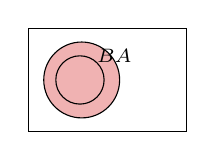
\begin{tikzpicture}[scale=.438]
\draw (-2,-2) rectangle (2.6,1);
\scope % A \cap B
\filldraw[fill=red!80!black!30] (-.45,-.5) circle (1.1);
\draw[fill=red!80!black!30] (-.5,-.5) circle (.7);
\endscope
\tkzText(-1.6,-1.6){{\scriptsize $ \varOmega $}}
\tkzText(.9,.1){{\scriptsize $ B $}}
\tkzText(-.45,-.2){{\scriptsize $ A $}}
\end{tikzpicture}} \\ 
\rule[-2ex]{0pt}{8.5ex} $ x\in\left(A\cap B\right)' $ & Συμπλήρωμα τομής & \textbf{Δεν} πραγματοποιούνται \textbf{συγχρονως} τα ενδ. $ A $ και $ B $. & \parbox[c]{22mm}{\mbox{}\\\begin{venndiagram2sets}[tikzoptions={scale=.4},shade=red!80!black!30,labelA={{\scriptsize $ A $}},labelB={{\scriptsize $ B $}},labelNotAB={{\scriptsize $ \varOmega $}}]
\fillNotAorNotB
\end{venndiagram2sets}}\\
\rule[-2ex]{0pt}{8.5ex} $ x\in\left(A\cup B\right)' $ & Συμπλήρωμα ένωσης & Δεν πραγματοποιείται \textbf{κανένα} από τα ενδ. $ A $ και $ B $. & \parbox[c]{22mm}{\mbox{}\\\begin{venndiagram2sets}[tikzoptions={scale=.4},shade=red!80!black!30,labelA={{\scriptsize $ A $}},labelB={{\scriptsize $ B $}},labelNotAB={{\scriptsize $ \varOmega $}}]
\fillNotAorB
\end{venndiagram2sets}}\\
\rule[-2ex]{0pt}{8.5ex} $ x\in\left( A-B\right)'  $ & Συμπλήρωμα διαφοράς & \textbf{Δεν} πραγματοποιείται μόνο το ενδεχόμενο $ A $. & \parbox[c]{22mm}{\mbox{}\\\begin{venndiagram2sets}[tikzoptions={scale=.4},shade=red!80!black!30,labelA={{\scriptsize $ A $}},labelB={{\scriptsize $ B $}},labelNotAB={{\scriptsize $ \varOmega $}}]
\fillNotAorB \fillB
\end{venndiagram2sets}} \\
\rule[-2ex]{0pt}{8.5ex} $ x\in \left(B-A\right)'  $ & Συμπλήρωμα διαφοράς & \textbf{Δεν} πραγματοποιείται μόνο το ενδεχόμενο $ B $. & \parbox[c]{22mm}{\mbox{}\\\begin{venndiagram2sets}[tikzoptions={scale=.4},shade=red!80!black!30,labelA={{\scriptsize $ A $}},labelB={{\scriptsize $ B $}},labelNotAB={{\scriptsize $ \varOmega $}}]
\fillNotAorB \fillA
\end{venndiagram2sets}} \\
\rule[-2ex]{0pt}{8.5ex} $ x\in\left( \left(A-B\right)\cup\left(B-A\right)\right)'  $ & Συμπλήρωμα ένωσης διαφορών & \textbf{Δεν} πραγματοποιείται μόνο ένα από τα δύο σύνολα (ή κανένα από τα δύο ή και τα δύο). & \parbox[c]{22mm}{\mbox{}\\\begin{venndiagram2sets}[tikzoptions={scale=.4},shade=red!80!black!30,labelA={{\scriptsize $ A $}},labelB={{\scriptsize $ B $}},labelNotAB={{\scriptsize $ \varOmega $}}]
\fillNotAorB \fillACapB
\end{venndiagram2sets}} \\
\rule[-1ex]{0pt}{0ex} &&&\\
\hline
\end{longtable}
%#--------------------------------------------------